\chapter{Theoretical Framework}
\lhead{Chapter 2 \emph{Theoretical Framework}}
\label{chap:2}
%\autoref{chap:2}

\section{The problem of overpopulation}
\bigskip

%(Kind of intro about ways to deal?) The first accidental collision took place in 2009 between two communications satellites, the US commercial non-operational Iridium 33 and the Russian military Kosmos-2251. The number of debris that this collision left behind was 1,366 pieces with average size of 12.5cm and average weight 1.1kg. \cite{Kelso 2009}
It is benchmark 

%The problem of overpopulation and of the increasing number of space debris is that the possibility of impact between a debris and an operational functioning orbiting object is very high. --> Edw mention Letizia space 

%Vale orbital capacity (Vale san section? Giati to exw an aferei sto 1.2 Scope etc.)

%Rules? e.g. Every orbital plane has a certain capacity. Based on those, the future satellite constellations should work. In general, there are no rules about the capacity allocation!

---------------

\section{LEO: a favorable spot}
\bigskip
%LEO Low Earth Orbit. (Overview - Status?!)

The Low Earth Orbit (LEO) is a favorable spot for placing satellites for various reasons. It's proximity from Earth makes it possible to launch even CubeSats, since their fuel capacity is enough to be able to maintain their position and/or to de-orbit at the end of their mission. Specifically in the recent years more and more small satellites and/or CubeSats are placed in LEO and in large constellations. (Fig. \ref{launch_traffic_LEO}) The need of proliferated constellations is also linked to the low altitude of the LEO region. Namely, for larger coverage, a satellite should be either placed in a higher altitude, or the mission should engage more satellites in order to compensate the smaller field of view that one satellite offers.

++ The total number of operating satellites, as of 31.3.2020 including all the launches by that date is 2,666 with 1,918 being in LEO. \cite{UCS} 

**• Launch traffic into the LEO protected region is changing significantly, fuelled by the proliferation of small
payloads, i.e. below 10.0 kg in mass, during the last few years in terms of number, but not contributing
significantly to the mass. (ESA report p.77)

\begin{figure}
\centering
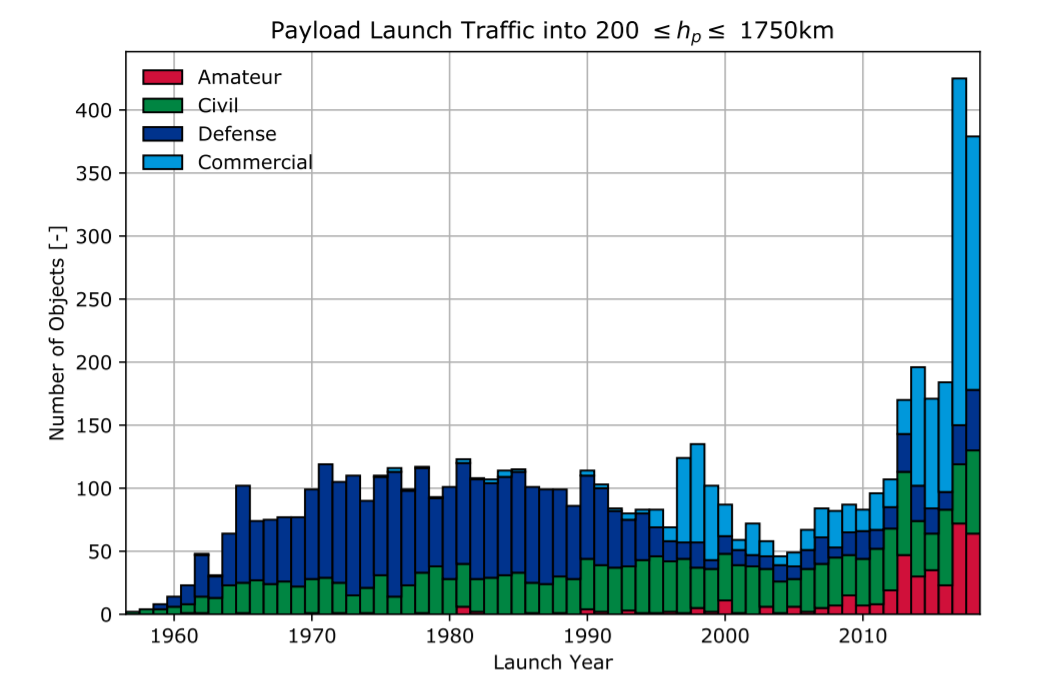
\includegraphics[width=0.9\textwidth]{Images/launch_traffic_LEO.png}\caption{Payload launch traffic into LEO (1957-2019). \textit{Source: \cite{ESA 2019}}}
\label{launch_traffic} 
\end{figure}

((Having said that, the current trend is that the world goes in the direction of launching more and more small satellites.))
This situation happens regardless of the overpopulation issues that exist in some regions of LEO, which has already been declared as critical. More specifically, the three critical regions in LEO are \cite{Kramer 2002}:
\begin{itemize}
\item The first critical region is at the altitude 750-850km, at which the spatial density is increased because of the debris' population. It is characterized as critical, because objects need hundreds of years in order to decay and re-enter the atmosphere.
\item The second critical region is at the altitude 900-1000km, at which there is a high number of massive objects. Drag is also not sufficient in order to help objects decay and thus the spatial density increases over time.
\item The third critical region is at the altitude 1100-1300km. At this region the effect of drag is negligible, which means that any additional object builds up the orbital population.
%The future large constellations will be placed around these altitudes, which makes this region even more alarming. \cite{Somma 2019}
\end{itemize}

%%Some general things about LEO:
%	General altitude range: 160-2000km above Earth’s surface.
%	Orbital periods between 88-127 min.
%	All inclinations possible
%	Orbital velocity (with regard to an observer on Earth): 7-8km/s
%	LEO subclasses/ “shapes”:
%•	Circular LEO orbit is the most common and natural orbit for Earth observation, especially in the altitude range of about 200-900 km with orbital periods of about 90-105min.
%•	Special orbits:
%	Polar orbit
%	Sun-Synchronous orbit (a special case of near-polar orbit!):
%An orbit like this is possible by the fact that the Earth is not a perfect sphere. In the SSO, the daily rotation of the orbital satellite plane (with respect to the equatorial plane) is identical to the mean motion of the fictitious sun around the Earth = which is identical to the mean motion of the Earth around the sun.
%	Check the relationship between the coverage and revisit/ repeat period with the inclination and altitude. (It’s on the application’s part.)


\subsection{Critical regions of LEO}
\bigskip

\section{Mitigation principles}
\bigskip

There have been made many important steps towards raising the consciousness about the overpopulation problem, as well as the enactment of rules regarding the capacity and orbit allocation. In 1993 the Inter-Agency Space Debris Coordination Committee (IADC) was founded. Some years later, in 2002 IADC published for the first time a report about Space Debris Mitigation Guidelines. These guidelines were presented at the United Nations Committee on the Peaceful Uses of Outer Space (UNCOPUOUS), which is a committee established by United Nations Office for Outer Space Affairs (UNOOSA). In 2003 another group working towards similar goals was created – the Orbital Debris Co-ordination Working Group (ODCWG), which was created by unanimous agreement of International Organization for Standardization (ISO). \cite{Klinkrad 2006}

Even though there are working groups (UNCOPUOUS, ODCWG) dealing with the mitigation guidelines, currently the existed space traffic management rules deal only with the frequency allocation used by satellites. For this reason, the motivation of this thesis is the creation of an application, which will help into supplementing the space traffic management rules regarding the physical location of satellites and the value added that they will contribute once launched.



--International cooperation at a technical level --
IADC (Inter-Agency Space Debris Coordination Committee) has declared protected regions \cite{IADC 2007}. "an inter-governmental forum whose aim is to co-ordinate efforts to deal with debris in orbit around the Earth founded in 1993." (It is composed of space agencies..)
%cite Space Debris: Models and Risk Analysis (978-3-540-37674-3) 


-- International standards and policies --
IADC also occupies a crucial role as a technical specialized group in the field of space debris since it supports the UNCOPUOUS.
The first publication related to the space debris mitigation was performed in 2002 by IADC and presented at UNCOPUOUS in 2003.

[[---> Also IADC guidelines (The UN Space Debris Mitigation Guidelines) --> Drafted on request of UNCOPUOUS (United Nations Committee on the Peaceful Uses of Outer Space), which is a committee established by UNOOSA (United Nations Office for Outer Space Affairs). \cite{IADC 2007}
1. Prevent the release of mission related object
2. Implement collision avoidance measures
3. Disposal
4. Passivation
5. Limit on-ground risk due to re-entry]]

The two main groups that they work towards these goals are the UNCOPUOUS working group and the Orbital Debris Co-ordination Working Group (ODCWG), which was created in 2003 by unanimous agreement of the ISO (International Organization for Standardization).

[[The recognized concepts from this meeting was that the mitigation of Orbital Space Debris is of international concern and the ISO is responsible for developing standards on a consensus basis.]]

